\section{Identifying weakly-coupled carbon-pins}
In order to understand how the features in the fingerprint from \cref{fig:FP} relate to the different spins and how this knowledge can be used to control these carbons it is necessary to understand what dynamical decoupling does to these atoms.

\subsection{The effect of dynamical decoupling}

\begin{figure}[htbp]
\centering
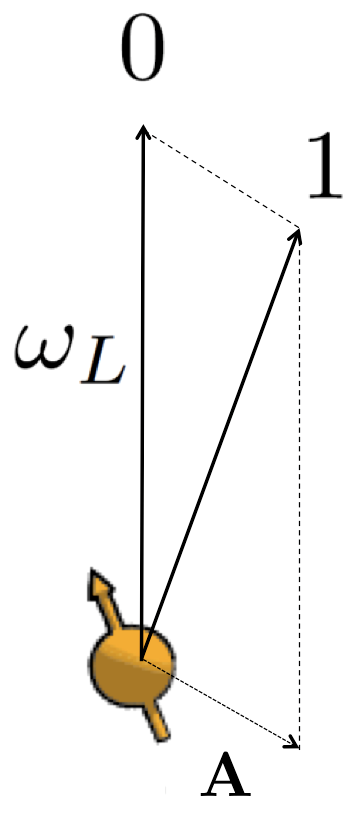
\includegraphics[keepaspectratio,width=0.15\textwidth]{./img/QuantizationAxis.png}
\caption{Flipping the electron spin from the  $m_s=0$ to the $m_s= +1$ state changes the quantization axis of nuclear spins. For  $m_s=0$ all nuclear spins precess about $\bm{\omega_L}$. For  $m_s=+1$ each spin precesses about a distinct axis $\bm{\tilde{\omega}}=\bm{\omega_L} +\bm{A}$.}
\label{fig:quantax}
\end{figure}

When the electron is in the $m_s=0$ state each nuclear spin precesses about $\bm{\omega_L}$ with the Larmor frequency. When the electron is in the $m_s=+1$ state nuclear spins precess about a distinct axis $\bm{\tilde{\omega}}=\bm{\omega_L} +\bm{A}$ \citep{Taminiau2012Detection}. The hyperfine interaction $\bm{A}$ depends on the position of that particular nuclear spin relative to the NV- center.

When applying a decoupling sequence with N\slash 2 decoupling units of the form {$\tau - \pi -2\tau-\pi-\tau$}, the nuclear spin alternately rotates around the  $\bm\omega_L$ and the $\bm{\tilde{\omega}}$ axis.
The net result of one such decoupling sequence is a rotation around an axis $\bm{\hat{\mathrm{n_i}}}$ by an angle $\phi$.
Where $\bm{\hat{\mathrm{n_i}}}$ depends on the initial state of the electron: $\bm{\hat{\mathrm{n_0}}}$ when the electron starts in $m_s = 0$ and $\bm{\hat{\mathrm{n_1}}}$ when the electron starts in $m_s = +1$~\citep{Taminiau2012Detection}.

\begin{figure}[htbp]
    \begin{subfigure}[t]{0.49\textwidth}\centering
        \centering
        \caption{}
        \includegraphics{Img/unCond_rot_taminiau.pdf}
        \label{fig:uncond_rot}
    \end{subfigure}
    \begin{subfigure}[t]{0.49\textwidth}\centering
        \centering
        \caption{}
        \includegraphics{Img/Cond_rot_taminiau.pdf}
        \label{fig:cond_rot}
    \end{subfigure}
    \caption{\Cref{fig:uncond_rot} When the net rotation axes $\bm{\hat{\mathrm{n_0}}}$ and $\bm{\hat{\mathrm{n_1}}}$ point in the same direction the carbon experiences an unconditional rotation and cannot be controlled. \Cref{fig:cond_rot} When the net rotation axes $\bm{\hat{\mathrm{n_0}}}$ and $\bm{\hat{\mathrm{n_1}}}$ are anti-parallel the carbon experiences a conditional rotation, either around +x or -x, and can be controlled.}
    \label{fig:conditional_and_unconditional_rotation}
\end{figure}


To understand how a carbon-13 atom can be controlled it is useful to consider three situations. In the first situation the $\bm{\omega_L}$ and $\bm{A}$ point in the same direction. In the second situation $\bm{\omega_L}$ and $\bm{A_\perp}$ are of comparable magnitude, resulting in a large angle between the quantization axes. In the last situation $|\bm{A}|$ is small compared to  $\bm{|\omega_L|}$ resulting in a small angle between the quantization axes.

When $\bm{\omega_L}$ and $\bm{A}$ point in the same direction, the net rotation axis is independent of the initial electron-state making it impossible to use the electron to control the carbon-13 atom using this decoupling sequence.

In the case where $\bm{\omega_L}$ and $\bm{A_\perp}$ are of comparable magnitude the net rotation axes $\bm{\hat{\mathrm{n_i}}}$ are strongly dependent on the initial electron-state for almost any $\tau$. This creates entanglement between the electron and this carbon for a wide range of inter pulse-delays $\tau$. For future reference we say that these weakly-coupled carbons are in the \emph{complex regime}.

When considering the case where the hyperfine interaction is much smaller than the Larmor frequency ($\omega_L \gg |\bm{A}|$), the net rotation axes  $\hat{\mathrm{n_0}}$ and $\hat{\mathrm{n_1}}$ are practically parallel and the nuclear spin undergoes an unconditional evolution.
Only when the inter-pulse delay is precisely resonant with the spin dynamics the axes are anti-parallel leading to a conditional rotation\citep{Taminiau2012Detection}.
The resonant condition is given by \cref{eq:res_dip_loc}, where $k$ is an integer and the FWHM of the Lorentzian-shaped resonance is given by \cref{eq:res_dip_width}.
To distinguish these carbons from those in the complex regime we say that these weakly-coupled carbons are in the \emph{basic regime}.

% somehow state that resonance gives a dip.
 \begin{equation}
\tau = \frac{(2k+1)\pi}{2 \omega_L + A_\parallel}
\label{eq:res_dip_loc}
\end{equation}
 \begin{equation}
\Delta = \frac{A_\perp}{2 \omega_L^2}
\label{eq:res_dip_width}
\end{equation}

If  $\hat{n_0}$ and $\hat{n_1}$ are not parallel, the resulting conditional rotation of the nuclear spin generally entangles the electron and nuclear spins.


\subsection{Response of a carbon-spin to dynamical decoupling spectroscopy}

As a result the electronic spin, starting out in $\ket{X}$, entangles with the nuclear spin for specific values of $\tau$ during a dynamical decoupling spectroscopy. %NOTE DOES NOT ENTANGLE NECCESARILY
When reading out the electronic spin along the X-axis this creates a dip in the signal.
The probability that the initial state is preserved is given by \cref{eq:contrast_to_probability}. Where the contrast $M_j$ for a single nuclear spin is given by \cref{eq:contrast_single_carbon_spin}\citep{Taminiau2012Detection}.

\begin{equation}
\label{eq:contrast_to_probability}
P_x = (M+1)/2
\end{equation}

\begin{equation}
\label{eq:contrast_single_carbon_spin}
M_j = 1-(1 - \hat{\bm{\mathrm{n_0}}} \cdot \hat{\bm{\mathrm{n_1}}}) \sin^2 \frac{N\phi}{2}
\end{equation}

%alpha = \tilde{\omega} \tau
%beta = (\omega_L \tau)
% mz = (\frac{ A_ \parallel + \omega_L }{ \tilde{ \omega}})
\begin{equation}
\label{eq:vec_term}
    1 - \hat{\bm{\mathrm{n_0}}} \cdot \hat{\bm{\mathrm{n_1}}} =  \frac{A_\perp ^2}{\tilde{\omega^2}} \frac{(1- \cos{(\tilde{\omega} \tau)})(1-\cos{(\omega_L \tau)})} {1 +\cos{(\tilde{\omega} \tau)}\cos{(\omega_L \tau)} - (\frac{ A_ \parallel + \omega_L }{ \tilde{ \omega}}) \sin{(\tilde{\omega} \tau)}\sin{(\omega_L \tau)}}
\end{equation}
\begin{equation}
\label{eq:angle_term}
    \phi =  \cos^{-1}\left(\cos(\tilde{\omega} \tau) \cos(\omega_L \tau)-\left(\frac{ A_ \parallel + \omega_L }{ \tilde{ \omega}}\right) \sin(\tilde{\omega} \tau)\sin(\omega_L \tau)\right)
\end{equation}
In reality the electron is not interacting with a single carbon but with a bath of carbon atoms. When the electron interacts with multiple carbons at the same time the contrast $M$ is given by the product of all individual values $M_j$ for each individual spin $j$ (\cref{eq:prod_multiple_spins}). In order to selectively control one carbon the electron should not entangle with any other carbon when addressing it.

\begin{equation}
\label{eq:prod_multiple_spins}
    M = \prod_{j}{M_j}
\end{equation}

When entanglement is created with multiple carbons at the same time coherence is quickly lost and contrast drops to 0.
By sweeping the number of pulses $\pi$-pules the response of an individual carbon can be distinguished from the response of multiple spins.
Only when an individual carbon is being addressed is it possible to sweep the contrast to -1.


\subsection{Identifying Individual Carbon-spins}

By identifying distinct dips in the fingerprint, of which \cref{fig:FP} shows a small part, we are able to make a first estimate of the hyperfine coupling using their location(\cref{eq:res_dip_loc}) and their width (\cref{eq:res_dip_width}.
We then compute the responses for these estimated hyperfine parameters using \cref{eq:contrast_single_carbon_spin}.
The parameters are varied until the computed response agrees with the data as well as possible to arrive at a more accurate estimation of the hyperfine parameters.
Using this method 13 distinct carbon spins where identified.

The parameters of the 4 strongest coupled carbons are listed in \cref{tbl:HF_par} and their computed responses are visible as colored lines in \cref{fig:FP}.
All estimated hyperfine parameters and a link to the full fingerprint measurements can be found in \cref{chap:Fingerprint_data_appendix}.

\begin{table}[htbp]
\centering
    \begin{tabular}{cllll}
    Carbon & \quad \quad  $A_{\parallel} $ & \quad \quad $A_{\perp}$ \\ \hline
    1         & $2 \pi \cdot${ }30.0 kHz             & $2 \pi \cdot${ }80.0 kHz                \\
    2         & $2 \pi \cdot${ }27.0 kHz             & $2 \pi \cdot${ }28.5 kHz              \\
    3         & $2 \pi \cdot$-51.0 kHz          & $2 \pi \cdot$105.0 kHz              \\
    4         & $2 \pi \cdot${ }45.1 kHz           & $2 \pi \cdot${ }20.0 kHz                \\
    \end{tabular}
    \caption{Estimated hyperfine parameters for spins 1 to 4 in \cref{fig:FP}.}
    \label{tbl:HF_par}
\end{table}



Most spins are relatively far away from the NV-center and have similar hyperfine couplings causing their resonances to overlap. This causes a broad feature with low coherence known as the spin-bath collapse. This feature is clearly visible in the fingerprint (\cref{fig:FP}) at $\tau/(4\tau_L) = m$ for odd $m$, where $\tau_L$ is the Larmor period ($\tau_L = \frac{2\pi}{\omega_L} $).

Spins that have a stronger than average hyperfine-interaction show up outside or at the edge of the spin-bath collapse.
Spins that are in the basic regime show up as a narrow dip.
Going to larger $\tau$ separates these dips further as the order of the resonance $k$ increases.
By looking at larger $\tau$ it is possible to resolve and address more resonances.
Several spins in the basic regime have been identified 3 of these are visible as colored lines in \cref{fig:FP}.
As computations are fundamentally limited by the coherence time there is a limit to the resonance-order that can be used to address carbons, making it impossible to resolve all weakly coupled spins.

Besides the carbons in the basic regime there are also weakly-coupled carbons that are more strongly coupled.
When a carbon in the complex regime is present in the NV-center this manifests itself as a resonance with strong oscillations on the side. Such a feature is also clearly visible in \cref{fig:FP}. We have identified the oscillations in the fingerprint as belong to a single spin which is denoted by the red line.

When a weakly coupled carbon in the complex regime is present a significant part of the fingerprint spectrum is inaccessible for controlling other carbons making them an undesired feature when attempting to control weakly coupled carbon spins.


\subsection{Effect of the magnetic field}

There are significant advantages to increasing the magnetic field when attempting to address weakly coupled carbons.
By increasing the magnetic field the Larmor frequency can be increased, reducing the number of carbons that are in the complex regime.
This causes the broad oscillating resonances to disappear allowing more carbons to be addressed.

Although increasing the magnetic field can improve the situation it is not always possible or desired.
When the magnetic field becomes too strong too strong the resonances become narrower than the resolution of the Arbitrary Waveform Generator used to generate the pulses that address the resonances, making it impossible to address these resonances effectively.
Simulations were performed (see \cref{chap:addressable_carbon_sims}) that indicate that for a natural carbon-13 concentration there is a range between 400G and 1400G where the magnetic field is optimal for controlling weakly coupled spins.

Besides the spin environment there are other factors affecting the choice for magnetic field.
Because the optical transitions used for readout and initialization depend on strain and magnetic field field\citep{Hensen2011MeasurementBased}, care must be taken when measuring that states do not mix in the excited state.
This combined with the fact that few experiments have been performed at high magnetic field and low temperature make it more practical to settle for a more moderate magnetic field of 300G.


